\documentclass{article} % For LaTeX2e

\usepackage{nips14submit_e,times}
\usepackage{hyperref}
\usepackage{url}
\usepackage{graphicx}

\usepackage{listings}
\usepackage{color}

\definecolor{lightgray}{rgb}{1,1,1}
\definecolor{darkgray}{rgb}{.4,.4,.4}
\definecolor{redstrings}{rgb}{0.64,0.08,0.08}
\definecolor{blue}{rgb}{0,0,1}
\definecolor{greencomments}{rgb}{0,0.5,0}
\definecolor{cyan}{rgb}{0.0,0.6,0.6}

\renewcommand{\lstlistingname}{Code fragment}


\lstdefinelanguage{JavaScript}{
  keywords={break, case, catch, continue, debugger, default, delete, do, else, finally, for, function, if, in, instanceof, new, return, switch, this, throw, try, typeof, var, void, while, with, null},
  keywordstyle=\color{blue}\bfseries,
  ndkeywords={class, export, boolean, throw, implements, import, this},
  ndkeywordstyle=\color{blue}\bfseries,
  identifierstyle=\color{black},
  sensitive=false,
  comment=[l]{//},
  morecomment=[s]{/*}{*/},
  commentstyle=\color{greencomments}\ttfamily,
  stringstyle=\color{redstrings}\ttfamily,
  morestring=[b]',
  morestring=[b]"
}

\lstset{
   language=JavaScript,
   backgroundcolor=\color{lightgray},
   extendedchars=true,
   basicstyle=\footnotesize\ttfamily,
   showstringspaces=false,
   showspaces=false,
   numbers=left,
   numberstyle=\footnotesize,
   numbersep=9pt,
   tabsize=2,
   breaklines=true,
   showtabs=false,
   captionpos=b
}


%\documentstyle[nips14submit_09,times,art10]{article} % For LaTeX 2.09


\title{QMiner – Data Analytics Platform for Processing Streams of Structured and Unstructured Data}


\author{
Blaz Fortuna, Jan Rupnik, Carolina Fortuna, Marko Grobelnik, \\
Viktor Jovanoski, Mario Karlovcec, Blaz Kazic, Klemen Kenda, \\
Gregor Leban, Jost Novljan, Miha Papler, Luis Rei, Blaz Sovdat, \\
Luka Stopar, Andrej Muhic \\
Department of Computer Science\\
Jožef Stefan Institute\\
Jamova cesta 39, Ljubljana, Slovenia \\
}

% The \author macro works with any number of authors. There are two commands
% used to separate the names and addresses of multiple authors: \And and \AND.
%
% Using \And between authors leaves it to \LaTeX{} to determine where to break
% the lines. Using \AND forces a linebreak at that point. So, if \LaTeX{}
% puts 3 of 4 authors names on the first line, and the last on the second
% line, try using \AND instead of \And before the third author name.

\newcommand{\fix}{\marginpar{FIX}}
\newcommand{\new}{\marginpar{NEW}}

% \nipsfinalcopy % Uncomment for camera-ready version

\begin{document}


\maketitle

\begin{abstract}
   QMiner is an open source analytics platform for performing large scale data analysis. The paper presents the main features, capabilities and design choices of the library, which is followed by examples.
\end{abstract}

\section{Introduction}
   QMiner grew out of projects in the areas of text, web and stream mining that Artificial Intelligence group at Jo\v{z}ef Stefan Institute was involved in over the last couple of years. We wanted developed solutions to be interactive and operate in real-time on data sets of hundreds of gigabytes while still using the computational resources we have available. These goals and constraints resulted in a unique set of features that we implemented in QMiner.
   QMiner applications are implemented in JavaScript, making it easy for novice users to get started. Using the JavaScript API it is easy to compose complete data processing pipelines and integrate with other systems via RESTful web services. The backend is implemented in C++ and can be included as a library into custom C++ projects, thus providing them with stream processing and data analytics capabilities.
   QMiner is available as open source project on GitHub under AGPL licence. The repository contains source code, introduction guide and complete documentations of QMiner JavaScript APIs.

\section{Features}
   Connecting storage, indexing and analytics --- QMiner stores and indexes the data in a way that makes the implemented machine learning methods more scalable. Computing feature vectors from stored records tries to reduce any duplication of data in the process and relies heavily on the integrated indexing and its features (e.g. probabilistic joins) to make the transformations faster. Data schemas provide types for directly storing vectors and sparse vectors as part of records.
   
   Multimodal data support --- QMiner provides native support for handling and learning from unstructured data such as text or graphs. For example, full text search, aggregation over text fields, creating and storing bag-of-words vectors directly in the data stores, and full integration of Stanford graph analysis library SNAP in the C++ and JavaScript APIs
   
   Processing streaming data --- QMiner provides building blocks for processing and learning from streams of text documents, website logs or numeric streams. For example, pipeline-able stream aggregates for maintaining aggregate statistics over the stream, and machine learning algorithms for learning from stream.
   
   Probabilistic joins between tables --- For some operations computing a complete join between tables is not necessary. For example, to compute the gender distribution of visitors of a particular web page, we do not really need a complete list of visitors for that particular web page. What suffices is a statistically representative sample. QMiner supports several sampling techniques for achieving this, and integrates the support for probabilistic joins in query language and feature extractors.


\section{Examples}
   QMiner lets you get from data to working models exposed through web service API in less than an hour. Most applications can be scripted fully in the JavaScript layer, taking advantage of components implemented in C++ and libraries such as Intel MKL.

   \subsection{Text processing, classification and regression}
      The example in this section demonstrates how to extract features from the movie dataset to build classification and regression models to predict movie genre and rating. 
      
      First, we import the analytics module which provides machine learning algorithms. Next, we load the data and enumerate features we would like to extract from the data set. For each feature we need to specify its type (for example, \texttt{text}), its source (for example, \texttt{Movies}), and name (for example, \texttt{plot}). (Source is the \emph{data store} from which we want to extract the feature; data store very roughly corresponds to table in relational databases.) We can now run batch learner that returns the model that tries to predict movie genres using the whole data set for training (in this case, the model is stored in the \texttt{genreModel} variable). Once we saved the model we can easily use it for prediction (for example, \texttt{var newGenre = genreModel.predict(newMovie);}). 

      \begin{lstlisting}[caption={Text mining: storage, feature extraction, classification and regression}] 	
      // Import analytics module
      var analytics = require("analytics.js");
      // Loading in the dataset.
      qm.load.jsonFile(Movies, "./sandbox/movies/movies.json");
       	
      // Declare the features we will use to build genre classification models
      var genreFeatures = [
          { type: "text", source: "Movies", field: "Title" },
          { type: "text", source: "Movies", field: "Plot" },
          { type: "join", source: { store: "Movies", join: "Actor" } },
          { type: "join", source: { store: "Movies", join: "Director"} }
      ];
      // Create a model for the Genres field, using all the movies as training set.
      var genreModel = analytics.newBatchModel(Movies.recs,
                          genreFeatures, Movies.field("Genres"));
      // Predict genres of a new movie
      var newMovie = qm.store("Movies").newRec(/*{...}*/);
      var result = genreModel.predict(newMovie);
      \end{lstlisting}

   \subsection{Time series processing}
      The following example demonstrates how to perform time series resampling, feature vector computation and prediction.

      \begin{figure}[h]
      \begin{center}
      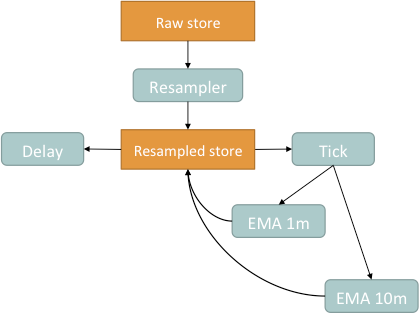
\includegraphics[width=0.5\textwidth]{timeSeries.png}
      \end{center}
      \caption{Time series processing architecture}
      \end{figure}

      \begin{lstlisting}[caption=Time series processing] 	
      // Initialize resamper from Raw to Resampled store. This results in
      // in an equaly spaced time series with 10 second interval.
      Raw.addStreamAggr({
          name: "Resample10second", type: "resampler",
          outStore: "Resampled", timestamp: "Time",
          fields: [{ name: "Value", interpolator: "previous" }],
          createStore: false, interval: 10 * 1000
      });
      // Initialize stream aggregates on Resampled store for computing
      // 1 minute and 10 minute exponential moving averages.
      Resampled.addStreamAggr({
          name: "tick", type: "timeSeriesTick",
          timestamp: "Time", value: "Value"
      });
      Resampled.addStreamAggr({
          name: "ema1m", type: "ema",
          inAggr: "tick", emaType: "previous", interval: 60000
      });
      Resampled.addStreamAggr({
          name: "ema10m", type: "ema",
          inAggr: "tick", emaType: "previous", interval: 600000
      });
      // Buffer for keeping track of the record from 1 minute ago
      Resampled.addStreamAggr({ name: "delay", type: "recordBuffer", size: 6 });

      // Declare features from the resampled timeseries
      var ftrSpace = analytics.newFeatureSpace([
          { type: "numeric", source: "Resampled", field: "Value" },
          { type: "numeric", source: "Resampled", field: "Ema1" },
          { type: "numeric", source: "Resampled", field: "Ema2" },
          { type: "multinomial", source: "Resampled", field: "Time", datetime: true }
      ]);
      // Initialize linear regression model.
      var linreg = analytics.newRecLinReg({ dim: ftrSpace.dim, forgetFact: 1.0 });
      // We register a trigger to Resampled store
      Resampled.addTrigger({
          onAdd: function (val) {
              // Get the latest value for EMAs
              val.Ema1 = Resampled.getStreamAggr("ema1m").val.Val;
              val.Ema2 = Resampled.getStreamAggr("ema10m").val.Val;
              // Get the id of the record from a minute ago.
              var trainRecId = Resampled.getStreamAggr("delay").val.last;;
              // Update the model
              linreg.learn(ftrSpace.ftrVec(Resampled[trainRecId]), val.Value);
          }
      });

      \end{lstlisting}

   \subsection{Graph analysis}


\section{Conclusions}
   Concluding remarks.

\subsubsection*{Acknowledgments}
   The authors gratefully acknowledge that the funding for this work was provided by the project X-LIKE (ICT-257790-STREP)\cite{xlike}.


\bibliographystyle{unsrt}
\bibliography{qminer}

\end{document}
